\documentclass[11pt]{article}

\usepackage{float}
% NOTE: Add in the relevant information to the commands below; or, if you'll be using the same information frequently, add these commands at the top of paolo-pset.tex file. 
\newcommand{\name}{Agustin Esteva}
\newcommand{\email}{aesteva@uchicago.edu}
\newcommand{\classnum}{13210}
\newcommand{\subject}{SSI: Formal Theory}
\newcommand{\instructors}{Scott Gehlbach}
\newcommand{\assignment}{Problem Set 4}
\newcommand{\semester}{Winter 2024}
\newcommand{\duedate}{2024-02-03}
\newcommand{\bA}{\mathbf{A}}
\newcommand{\bB}{\mathbf{B}}
\newcommand{\bC}{\mathbf{C}}
\newcommand{\bD}{\mathbf{D}}
\newcommand{\bE}{\mathbf{E}}
\newcommand{\bF}{\mathbf{F}}
\newcommand{\bG}{\mathbf{G}}
\newcommand{\bH}{\mathbf{H}}
\newcommand{\bI}{\mathbf{I}}
\newcommand{\bJ}{\mathbf{J}}
\newcommand{\bK}{\mathbf{K}}
\newcommand{\bL}{\mathbf{L}}
\newcommand{\bM}{\mathbf{M}}
\newcommand{\bN}{\mathbf{N}}
\newcommand{\bO}{\mathbf{O}}
\newcommand{\bP}{\mathbf{P}}
\newcommand{\bQ}{\mathbf{Q}}
\newcommand{\bR}{\mathbf{R}}
\newcommand{\bS}{\mathbf{S}}
\newcommand{\bT}{\mathbf{T}}
\newcommand{\bU}{\mathbf{U}}
\newcommand{\bV}{\mathbf{V}}
\newcommand{\bW}{\mathbf{W}}
\newcommand{\bX}{\mathbf{X}}
\newcommand{\bY}{\mathbf{Y}}
\newcommand{\bZ}{\mathbf{Z}}
\newcommand{\Var}{\text{Var}}

%% blackboard bold math capitals
\newcommand{\bbA}{\mathbb{A}}
\newcommand{\bbB}{\mathbb{B}}
\newcommand{\bbC}{\mathbb{C}}
\newcommand{\bbD}{\mathbb{D}}
\newcommand{\bbE}{\mathbb{E}}
\newcommand{\bbF}{\mathbb{F}}
\newcommand{\bbG}{\mathbb{G}}
\newcommand{\bbH}{\mathbb{H}}
\newcommand{\bbI}{\mathbb{I}}
\newcommand{\bbJ}{\mathbb{J}}
\newcommand{\bbK}{\mathbb{K}}
\newcommand{\bbL}{\mathbb{L}}
\newcommand{\bbM}{\mathbb{M}}
\newcommand{\bbN}{\mathbb{N}}
\newcommand{\bbO}{\mathbb{O}}
\newcommand{\bbP}{\mathbb{P}}
\newcommand{\bbQ}{\mathbb{Q}}
\newcommand{\bbR}{\mathbb{R}}
\newcommand{\bbS}{\mathbb{S}}
\newcommand{\bbT}{\mathbb{T}}
\newcommand{\bbU}{\mathbb{U}}
\newcommand{\bbV}{\mathbb{V}}
\newcommand{\bbW}{\mathbb{W}}
\newcommand{\bbX}{\mathbb{X}}
\newcommand{\bbY}{\mathbb{Y}}
\newcommand{\bbZ}{\mathbb{Z}}

%% script math capitals
\newcommand{\sA}{\mathscr{A}}
\newcommand{\sB}{\mathscr{B}}
\newcommand{\sC}{\mathscr{C}}
\newcommand{\sD}{\mathscr{D}}
\newcommand{\sE}{\mathscr{E}}
\newcommand{\sF}{\mathscr{F}}
\newcommand{\sG}{\mathscr{G}}
\newcommand{\sH}{\mathscr{H}}
\newcommand{\sI}{\mathscr{I}}
\newcommand{\sJ}{\mathscr{J}}
\newcommand{\sK}{\mathscr{K}}
\newcommand{\sL}{\mathscr{L}}
\newcommand{\sM}{\mathscr{M}}
\newcommand{\sN}{\mathscr{N}}
\newcommand{\sO}{\mathscr{O}}
\newcommand{\sP}{\mathscr{P}}
\newcommand{\sQ}{\mathscr{Q}}
\newcommand{\sR}{\mathscr{R}}
\newcommand{\sS}{\mathscr{S}}
\newcommand{\sT}{\mathscr{T}}
\newcommand{\sU}{\mathscr{U}}
\newcommand{\sV}{\mathscr{V}}
\newcommand{\sW}{\mathscr{W}}
\newcommand{\sX}{\mathscr{X}}
\newcommand{\sY}{\mathscr{Y}}
\newcommand{\sZ}{\mathscr{Z}}


\renewcommand{\emptyset}{\O}

\newcommand{\abs}[1]{\lvert #1 \rvert}
\newcommand{\norm}[1]{\lVert #1 \rVert}
\newcommand{\sm}{\setminus}


\newcommand{\sarr}{\rightarrow}
\newcommand{\arr}{\longrightarrow}

% NOTE: Defining collaborators is optional; to not list collaborators, comment out the line below.
%\newcommand{\collaborators}{Alyssa P. Hacker (\texttt{aphacker}), Ben Bitdiddle (\texttt{bitdiddle})}

\input{paolo-pset.tex}

% NOTE: To compile a version of this pset without problems, solutions, or reflections, uncomment the relevant line below.

%\excludeversion{problem}
%\excludeversion{solution}
%\excludeversion{reflection}

\begin{document}	
	
	% Use the \psetheader command at the beginning of a pset. 
	\psetheader
\section*{Problem 1}
Consider the following extensive game with perfect information.

\begin{center}
    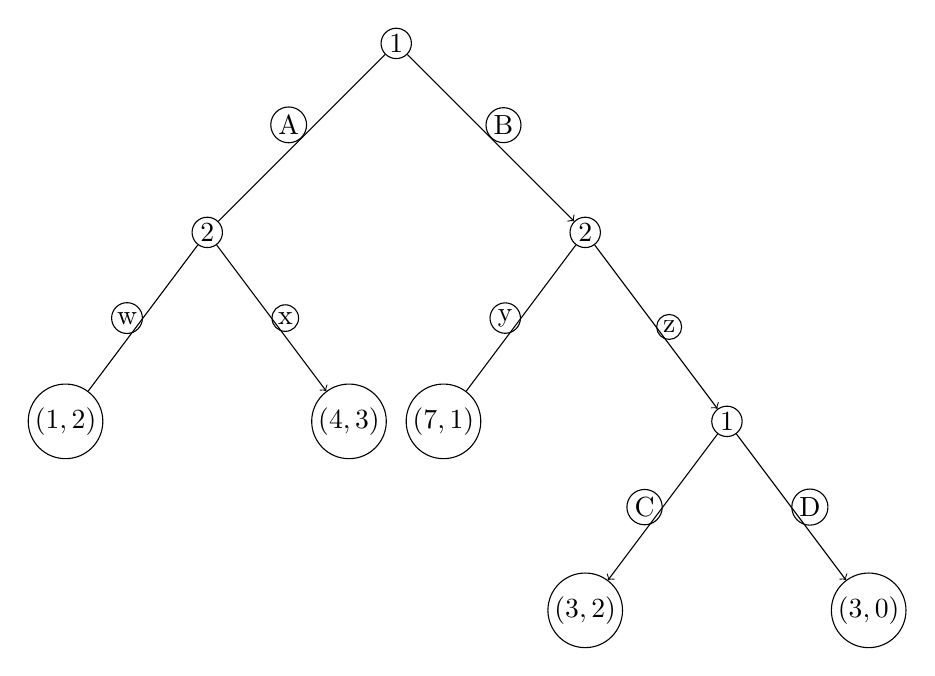
\begin{tikzpicture}[scale=1.2, every node/.style={draw, circle, inner sep=1pt}]
        \node (A) at (0,0) {1};
        \node (B) at (-2,-2) {2};
        \node (C) at (2,-2) {2};
        \node (D) at (-3.5,-4) {$(1,2)$};
        \node (E) at (-0.5,-4) {$(4,3)$};
        \node (F) at (0.5,-4) {$(7,1)$};
        \node (G) at (3.5,-4) {1};
        \node (L) at (2,-6) {$(3,2)$};
        \node (M) at (5,-6) {$(3,0)$};

        \draw (A) -- (B) node[midway, above left] {A};
        \draw[->] (A) -- (C) node[midway, above right] {B};
        \draw (B) -- (D) node[midway, left] {w};
        \draw[->] (B) -- (E) node[midway, right] {x};
        \draw (C) -- (F) node[midway, left] {y};
        \draw[->] (C) -- (G) node[midway, right] {z};
        \draw[->] (G) -- (L) node[midway, left] {C};
        \draw[->] (G) -- (M) node[midway, right] {D};
    \end{tikzpicture}
\end{center}

\begin{enumerate}
    \item[(a)] Write down the strategic form and find all Nash equilibria. For each equilibrium, find the equilibrium outcome. (Be sure you understand the difference.)
    \begin{solution}
    Strategic Form:
    \begin{table}[H]
        \centering
        \begin{tabular}{|c|c|l|l|l|} \hline 
 & wy&wz &xy &xz\\ \hline 
AC& 1,2& 1,2& 4,\textbf{3}&\textbf{4},\textbf{3}\\ \hline 
AD& 1,2&  1,2& 4,\textbf{3}&\textbf{4},\textbf{3}\\ \hline
BC& \textbf{7},1& \textbf{3},\textbf{2}& 7,1&3,\textbf{2}\\\hline
BD& \textbf{7},\textbf{1}& \textbf{3},0& \textbf{7},\textbf{1}&3,0\\\hline\end{tabular}
        \caption{Strategic Form}
    \end{table}
    From best response method in table above:
    \[\boxed{s = (AC, xz) \to O(s) = (A,x)} \]
    \[\boxed{s = (AD, xz) \to O(s) = (A,x)}\]
    \[\boxed{s = (BC, wz) \to O(s) = (B,z ,C)}\]
    \[\boxed{s = (BD, wy) \to O(s) = (B,y)}\]
    \[\boxed{s = (BD, xy) \to O(s) = (B,y)}\]
        \end{solution}
    \item[(b)] Find all subgame-perfect Nash equilibria. For each equilibrium, provide the equilibrium outcome.
    \begin{solution}
    \begin{table}[H]
        \centering
        \begin{tabular}{c|cl}
 &Optimal action  &Optimal action  \\
             Subgame 1 (1, C,D)&  C&D\\
             Subgame 2 (2, w,x,y,x)& 
         xz&xy\\
 Subgame 3 (1, A,B)& A&B\\\end{tabular}
        \caption{Finding SPNE}
    \end{table}
        From the tree and the table above, we see that the SPNE are 
        \[\boxed{ s= \{(AC, xz), (BD, xy)\}}\]
        \[\boxed{O(s_1) = (A,x)}, \quad \boxed{O(s_2) = (B, y)}\]
    \end{solution}
    \item[(c)] How do your answers to parts (a) and (b) compare? Please explain the difference, if any.
    \begin{solution}
        There are strictly less SPNE than there are Nash Equilibria. The interesting thing to note is that in no strategy which results in player one playing twice is a SPNE. That is, player two knows it is not optimal for her to let player one go again. 
    \end{solution}
\end{enumerate}

\section*{Problem 2}
Consider the ultimatum bargaining game with two players, but now assume that the players are altruistic, in the sense that they value not only their own share of the resource but also (though to a lesser extent) the other player’s share. The following utility functions represent these preferences:

\begin{align*}
    u_1 (x_1, x_2) &= x_1 + \alpha x_2, \\
    u_2 (x_1, x_2) &= \alpha x_1 + x_2,
\end{align*}
where $\alpha \in (0,1)$. If bargaining breaks down (i.e., if player 2 rejects player 1’s offer), then the players receive default shares $\bar{x}_1 = \bar{x}_2 = 0$.

\begin{enumerate}
    \item[(a)] What offers will Player 2 accept?
    \begin{solution}
    Here, we assume the total resources are $1$ (normalize if not). 
    
        If player $2$ rejects, then he gets $0$ utility. Let $x_1 \in [0,1].$ Then since $\alpha \in (0,1),$ we have that
        \[u_2(x_1, x_2) = \alpha x_1 + (1-x_1) = 1 + x_1(\alpha -1) >0,\] and so player $2$ will accept no matter what. 
    \end{solution}
    \item[(b)] What is the subgame-perfect Nash equilibrium?
    \begin{solution}
        Since player $2$ always accepts, the subgame-perfect equilibria will arise when player $1$ chooses his best possible option. That is, when $u_1(x_1, x_2)$ is maximized:
        \[u_1(x_1 + x_2) = x_1 + \alpha(1 - x_1) \implies \hat{x}_1 = 1,\] and so the subgame perfect Nash Equilibrium is simply 
        \[\boxed{s = (x_1 = 1, \text{Accept})}\]
    \end{solution}
    \item[(c)] What is the equilibrium outcome?
    \begin{solution}
        From above, 
        \[\boxed{O(s) = (1, 0)}\]
    \end{solution}
\end{enumerate}

\section*{Problem 3}
Two people select a policy among three alternatives, $X$, $Y$, and $Z$, by alternately vetoing policies until only one remains: first, person 1 vetoes a policy, following which person 2 vetoes one of the two policies that remain. Suppose person 1 strictly prefers $X$ to $Y$ to $Z$, whereas person 2 strictly prefers $Z$ to $Y$ to $X$.

\begin{enumerate}
    \item[(a)] Model this situation as an extensive game with perfect information and ordinal preferences. Draw a picture.
    \begin{solution}
    Game tree:
    \[
        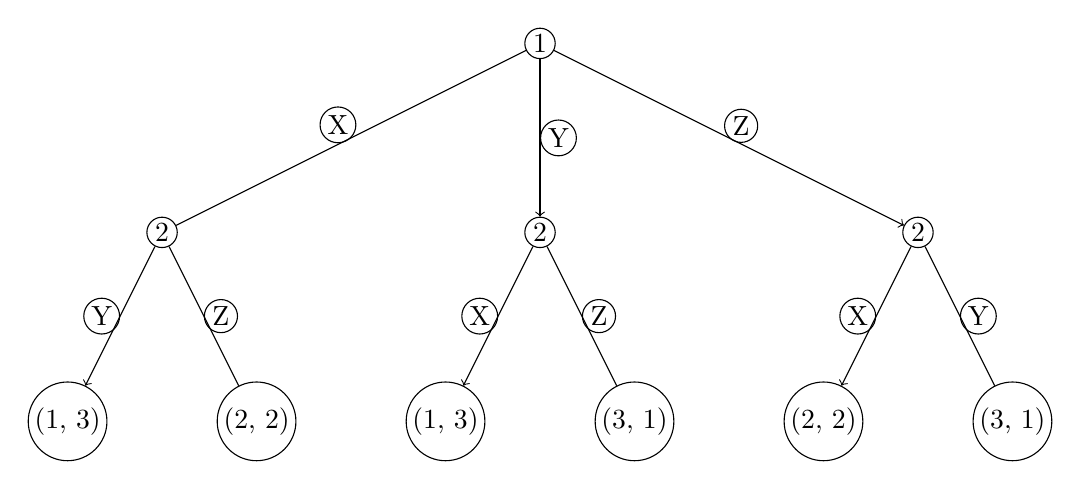
\begin{tikzpicture}[scale=1.2, every node/.style={draw, circle, inner sep=1pt}]
        \node (A) at (0,0) {1};
        
        \node (B) at (-4,-2) {2};
        \node (C) at (0,-2) {2};
        \node (D) at (4, -2) {2};
        
        \node (E) at (-5,-4) {(1, 3)};
        \node (F) at (-3,-4) {(2, 2)};

        \node (G) at (-1,-4) {(1, 3)};
        \node (H) at (1,-4) {(3, 1)};

        \node (I) at (3,-4) {(2, 2)};
        \node (J) at (5,-4) {(3, 1)};

        \draw (A) -- (B) node[midway, above left] {X};
        \draw (A) -- (C)[->] node[midway, right] {Y};
        \draw (A) -- (D)[->] node[midway, above right] {Z};

        \draw (B) -- (E)[->] node[midway, left] {Y};
        \draw (B) -- (F) node[midway, right] {Z};

        \draw (C) -- (G)[->] node[midway, left] {X};
        \draw (C) -- (H) node[midway, right] {Z};

        \draw (D) -- (I)[->] node[midway, left] {X};
        \draw (D) -- (J) node[midway, right] {Y};
    \end{tikzpicture}\]
    \end{solution}
    \item[(b)] For each of the two players, list all available strategies.
    \begin{solution}
        \[\boxed{S_1 = \begin{bmatrix}
            X\\Y\\Z
        \end{bmatrix}}\]
        \[\boxed{S_2 = \begin{bmatrix}
            YXX & YXY & YZX & YZY & ZXX & ZXY & ZZX & ZZY
        \end{bmatrix}}\]
    \end{solution}
    \item[(c)] Construct the strategic form of this game and find all Nash equilibria.
    \begin{solution}
        \begin{table}[H]
        \centering
        \begin{tabular}{|c|c|l|l|l|l|l|l|l|l} \hline 
  & YXX & YXY & YZX & YZY & ZXX & ZXY & ZZX &ZZY \\\hline 
X & 1,\textbf{3} & 1,\textbf{3} & 1,\textbf{3} & 1,\textbf{3} & \textbf{2},2 & 2,2 & 2,2 & 2,2 
    \\\hline 
Y & 1,\textbf{3} & 1,\textbf{3} & \textbf{3},1 & \textbf{3},1 & 1,\textbf{3} & 1,\textbf{3} & \textbf{3},1 &  \textbf{3},1
    \\\hline 
Z & \textbf{2},\textbf{2} & \textbf{3},1 & 2,\textbf{2} &\textbf{3},1 &\textbf{2},\textbf{2} &\textbf{3},1 & 2,\textbf{2} & \textbf{3},1
    \\\hline 
\end{tabular}
        \caption{Strategic Form}
    \end{table}
From best response method:
\[\boxed{s = (Z, YXX) \mapsto O(s) = (Z,X)}\]
\[\boxed{s = (Z, ZXX) \mapsto O(s) = (Z,X)}\]
    \end{solution}
    \item[(d)] Find all subgame-perfect Nash equilibria.
\begin{solution}
    \begin{table}[H]
        \centering
        \begin{tabular}{cl}
                                &Optimal action    \\
             Subgame 1 (2, $S_2$)&  YXX\\
             Subgame 2 (2, $S_1$)& Z
             \\\end{tabular}
        \caption{Finding SPNE}
    \end{table}
    From the arrows in the tree and the table above, we see that \[\boxed{s = (Z, YXX) \implies O(s) = (Z,X)}\] is the unique SPNE and the unique outcome.
\end{solution}
    \item[(e)] Does the game have any Nash equilibria that are not subgame-perfect Nash equilibria? Is any outcome of a Nash equilibrium not the outcome of some subgame-perfect Nash equilibrium?
    \begin{solution}
        The game has two Nash Equilibrium but only one SPNE. However, the game only has a single NE outcome, which corresponds of course to the SPNE outcome.
    \end{solution}
\end{enumerate}


















\end{document}